
% part 18

\section{Deferred'ы в целом\label{sec:part18}}

\subsection{Введение}


В предыдущей главе мы изучили новый способ структурирования 
последовтельных асинхронных callback'ов с использованием 
генератора. Таким образом, включая deferred'ы, у нас теперь две 
техники для связывания асинхронных операций вместе. 


Иногда нужно запустить группу асинхронных операций ``параллельно''. 
Поскольку Twisted однотредовый, то асинхронные операции 
реально не запускаются параллельно, мы просто указываем место, где  
хотим использовать асинхронный ввод-вывод. Например, наши поэтические 
клиенты скачивают поэмы из разных серверов одновременно, а не с одного 
сервера, а потом с другого.


Как узнать, что все асинхронные 
операции, которые были начаты, завершены? До сих пор 
мы решали эту задачу, собирая наши результаты в список (подобно 
\href{http://github.com/jdavisp3/twisted-intro/blob/master/twisted-client-7/get-poetry.py#L160}{списку результатов} 
в клиенте 7.0) и проверяли длину списка. 
Мы должны были тщательно собирать как успешные запуски, так и 
неуспешные, иначе один неуспешный запуск мог вызвать то, что программа 
запускалась всегда, предполагая, что еще остались незавершенные 
задачи.


Как вы догадываетесь, Twisted включает абстракцию, 
которую вы можете использовать для решения этой 
проблемы, и мы посмотрим на это в этой главе.


\subsection{DeferredList}

Класс \href{http://twistedmatrix.com/trac/browser/tags/releases/twisted-10.1.0/twisted/internet/defer.py#593}{DeferredList} позволяет нам обрабатывать список объектов типа Deferred как 
один deferred. Таким способом мы можем запустить пачку 
асинхронных операций и получить уведомление, только тогда, когда 
все они завершены (несмотря на успешный или ошибочный результат). 
Давайте рассмотрим несколько примеров.


В примере \href{http://github.com/jdavisp3/twisted-intro/blob/master/deferred-list/deferred-list-1.py#L1}{deferred-list/deferred-list-1.py} вы найдете следующий код:

\begin{scriptsize}\begin{verbatim}
from twisted.internet import defer

def got_results(res):
    print 'We got:', res

print 'Empty List.'
d = defer.DeferredList([])
print 'Adding Callback.'
d.addCallback(got_results)
\end{verbatim}\end{scriptsize}

Если вы запустите, то получите следующий вывод:

\begin{scriptsize}\begin{verbatim}
Empty List.
Adding Callback.
We got: []
\end{verbatim}\end{scriptsize}

Нужно отметить следующее:

\begin{itemize}

\item DefferedList создается из Python списка. В первом примере список 
    пустой, но мы увидим, что элементы списка должны быть объектами 
    типа Deffered.

\item DeferredList - сам является deferred'ом, так как унаследован от Deferred. Это означает, 
    что вы можете добавлять callback'и и errback'и в него, так, как будто 
    это обычный deferred.

\item В примере выше, наш callback был активизирован сразу же 
    после добавления, так что DeferredList должен активизироваться 
    сразу же. Мы обсудим это позже.

\item Результат deferred списка - список (пустой). 

\end{itemize}

Давайте теперь помотрим на 
\href{http://github.com/jdavisp3/twisted-intro/blob/master/deferred-list/deferred-list-2.py#L1}{deferred-list/deferred-list-2.py}:

\begin{scriptsize}\begin{verbatim}
from twisted.internet import defer

def got_results(res):
    print 'We got:', res

print 'One Deferred.'
d1 = defer.Deferred()
d = defer.DeferredList([d1])
print 'Adding Callback.'
d.addCallback(got_results)
print 'Firing d1.'
d1.callback('d1 result')
\end{verbatim}\end{scriptsize}


Теперь мы создаем DeferredList с одним элементом в 
списке. Получаем следующий вывод:

\begin{scriptsize}\begin{verbatim}
One Deferred.
Adding Callback.
Firing d1.
We got: [(True, 'd1 result')]
\end{verbatim}\end{scriptsize}

Нужно отметить следующее:

\begin{itemize}

\item На этот раз DeferredList не активизировал свой callback, 
    до тех пор пока мы не активизировали deferred в списке.

\item Результат - это все еще список, но теперь с одним элеметом.

\item Элемент в возвращенном списке - кортеж, у которого второе значение - 
    результат deferred'а в списке.

\end{itemize}

Давайте попробуем добавить два deferred'а в список(
\href{http://github.com/jdavisp3/twisted-intro/blob/master/deferred-list/deferred-list-1.py#L3}{deferred-list/deferred-list-3.py}):

\begin{scriptsize}\begin{verbatim}
from twisted.internet import defer

def got_results(res):
    print 'We got:', res

print 'Two Deferreds.'
d1 = defer.Deferred()
d2 = defer.Deferred()
d = defer.DeferredList([d1, d2])
print 'Adding Callback.'
d.addCallback(got_results)
print 'Firing d1.'
d1.callback('d1 result')
print 'Firing d2.'
d2.callback('d2 result')
\end{verbatim}\end{scriptsize}

Вывод следующий:

\begin{scriptsize}\begin{verbatim}
Two Deferreds.
Adding Callback.
Firing d1.
Firing d2.
We got: [(True, 'd1 result'), (True, 'd2 result')]
\end{verbatim}\end{scriptsize}


С этого момента достаточно ясен результат DeferredList, 
по меньшей мере способ, которым мы его использовали, - 
список элементов по количеству deferred'ов в списке, 
который мы передали в конструктор. И элементы списка 
результатов содержат результаты первоначальных deferred'ов, 
по меньшей мере deferred'ов, которые успешно завершились. 
Это означает, что сам по себе DeferredList не активизируется 
до тех пор пока все deferred'ы в списке не активизированы. И 
DeferredList, созданный с пустым списком, активизируется 
сразу же, поскольку нет deferred'в, завершения которых 
надо ожидать.


Что по поводу порядка резульатов в списке с результатами? 
Рассмотрим \href{http://github.com/jdavisp3/twisted-intro/blob/master/deferred-list/deferred-list-4.py#L1}{deferred-list/deferred-list-4.py}:

\begin{scriptsize}\begin{verbatim}
from twisted.internet import defer

def got_results(res):
    print 'We got:', res

print 'Two Deferreds.'
d1 = defer.Deferred()
d2 = defer.Deferred()
d = defer.DeferredList([d1, d2])
print 'Adding Callback.'
d.addCallback(got_results)
print 'Firing d2.'
d2.callback('d2 result')
print 'Firing d1.'
d1.callback('d1 result')
\end{verbatim}\end{scriptsize}

На этот раз мы активизировали сначала d2, а потом d1. Заметим, что 
список deferred'ов все еще создается с d1 и d2 в их 
первоначальном порядке. Далее вывод:

\begin{scriptsize}\begin{verbatim}
Two Deferreds.
Adding Callback.
Firing d2.
Firing d1.
We got: [(True, 'd1 result'), (True, 'd2 result')]
\end{verbatim}\end{scriptsize}


Результирующий список имеет результаты в то же самом порядке, что и 
первоначальный список deferred'ов, порядок не соответвует 
очередности запуска deferred'ов. Что очень хорошо, поскольку 
мы можем связать каждый индивидуальный результат с 
действием, которое их порождает (например, какая поэма с какого сервера пришла).


Что происходит, если один или более deferred'ов в списке 
завершились с ошибкой? И что здесь делают значения True? 
Давайте попробуем пример \href{http://github.com/jdavisp3/twisted-intro/blob/master/deferred-list/deferred-list-5.py#L1}{deferred-list/deferred-list-5.py}:

\begin{scriptsize}\begin{verbatim}
from twisted.internet import defer

def got_results(res):
    print 'We got:', res

d1 = defer.Deferred()
d2 = defer.Deferred()
d = defer.DeferredList([d1, d2], consumeErrors=True)
d.addCallback(got_results)
print 'Firing d1.'
d1.callback('d1 result')
print 'Firing d2 with errback.'
d2.errback(Exception('d2 failure'))
\end{verbatim}\end{scriptsize}

Теперь мы активизировали d1 c положительным результатом, а 
d2 - отрицательным. Игнорируя опцию consumerErrors, 
мы вернемся к этому, вывод будет следующий:

\begin{scriptsize}\begin{verbatim}
Firing d1.
Firing d2 with errback.
We got: [(True, 'd1 result'), (False, <twisted.python.failure.Failure <type 'exceptions.Exception'>>)]
\end{verbatim}\end{scriptsize}

Теперь кортеж соответсвующий d2 имеет Failure в качестве второго элемента и 
False - в качестве первого. С этого момента должно быть достаточно понятно, как 
работает DeferredList:

\begin{itemize}

\item DeferredList конструируется со списком объектов типа Deferred.

\item DeferredList сам deferred, с результатом ввиде списка той же длины, что и список deferred'ов.

\item DeferredList активизируется после того как все deferred'ы в первоначальном 
    списке активизированы.

\item Каждый элемент резуьтирующего списка соответсвует 
    deferred'у в той же позиции, что и в первоначальном списке. Если 
    deferred завершился успешно, то элемент - (True, result), 
    иначе - (False, failure).

\item DeferredList никогда не завершается с ошибкой, поскольку 
    результат каждого отдельного deferred'а собирается в список 
    в любом случае.
\end{itemize}


Давайте теперь поговорим об опции consumeErrors в 
конструкторе DeferredList. Если мы запускаем код 
\href{http://github.com/jdavisp3/twisted-intro/blob/master/deferred-list/deferred-list-6.py#L1}{deferred-list/deferred-list-6.py}, в котором не используется эта опция, вывод получается такой:


\begin{scriptsize}\begin{verbatim}
Firing d1.
Firing d2 with errback.
We got: [(True, 'd1 result'), (False, >twisted.python.failure.Failure >type 'exceptions.Exception'<<)]
Unhandled error in Deferred:
Traceback (most recent call last):
Failure: exceptions.Exception: d2 failure
\end{verbatim}\end{scriptsize}


Если вы вспомните, то сообщение ``Unhandled error in Deferred'' 
генерируется, когда deferred собирается сборщиком мусора, и 
последний callback в deferred'е завершился с ошибкой. Это сообщение 
говорит нам, что мы не поймали все потенциальные асинхронные 
ошибки в нашей программе. И откуда это приходит в нашем примере? 
Ясно, что это не приходит от DeferredList, посколько DeferredList 
всегда запускается успешно. Поэтому, это приходит от d2.


DeferredList нужно знать, когда каждый из deferred'ов, 
которые он мониторит, активизировались. И DeferredList 
делает это обычным образом - путем добавления 
callback и errback к каждому deferred'у. По умолчанию, 
callback (и errback) возвращают первоначальный 
результат (или ошибку) после их помещения в окончательный 
список. Возвращая первоначальный Failure из 
errback тригеров следующему errback, d2 остается в состоянии 
ошибки после активизации.


Но если мы подставляем consumeErrors=True в DeferredList, 
errback, добавленный в DeferredList для каждого 
deferred'а, возвратит None, таким образом потребляя ошибку и 
выдавая предуреждение. Мы также можем управлять ошибкой, добавляя 
свой собственный errback в d2, так как это делается в 
\href{http://github.com/jdavisp3/twisted-intro/blob/master/deferred-list/deferred-list-7.py#L1}{deferred-list/deferred-list-7.py}.


\subsection{Клиент 8.0}


В версии 8.0 поэтического клиента используется DeferredList 
для поиска, когда вся поэзия успешно завершилась (или 
завершилась с ошибкой). Новый поэтический клиент можно 
найти в \href{http://github.com/jdavisp3/twisted-intro/blob/master/twisted-client-8/get-poetry.py#L1}{twisted-client-8/get-poetry.py}. Изменения коснулись только poetry\_main. Давайте 
посмотрим на важные изменения:

\begin{scriptsize}\begin{verbatim}
    ...
    ds = []

    for (host, port) in addresses:
        d = get_transformed_poem(host, port)
        d.addCallbacks(got_poem)
        ds.append(d)

    dlist = defer.DeferredList(ds, consumeErrors=True)
    dlist.addCallback(lambda res : reactor.stop())
\end{verbatim}\end{scriptsize}


В клиенте 8.0 вам не нужен callback poem\_done или 
список результатов. Вместо этого, мы помещаем каждый 
deferred, который мы получаем от get\_transformed\_poem 
в список (ds) и затем создаем DeferredList. Посколько 
DeferredList не будет активизироваться до тех пор пока все 
поэмы не завершаться успешно или с ошибкой, мы добавляем 
в DeferredList callback, останавливающий reactor. В этом 
случае, мы не используем результат из DeferredList, мы только 
хотим знать, когда все завершилось.

\subsection{Обсуждение}

На рисунке \ref{fig:deferred-list} визуализация того, 
как работает DeferredList: 

\begin{figure}[h]
\begin{center}
    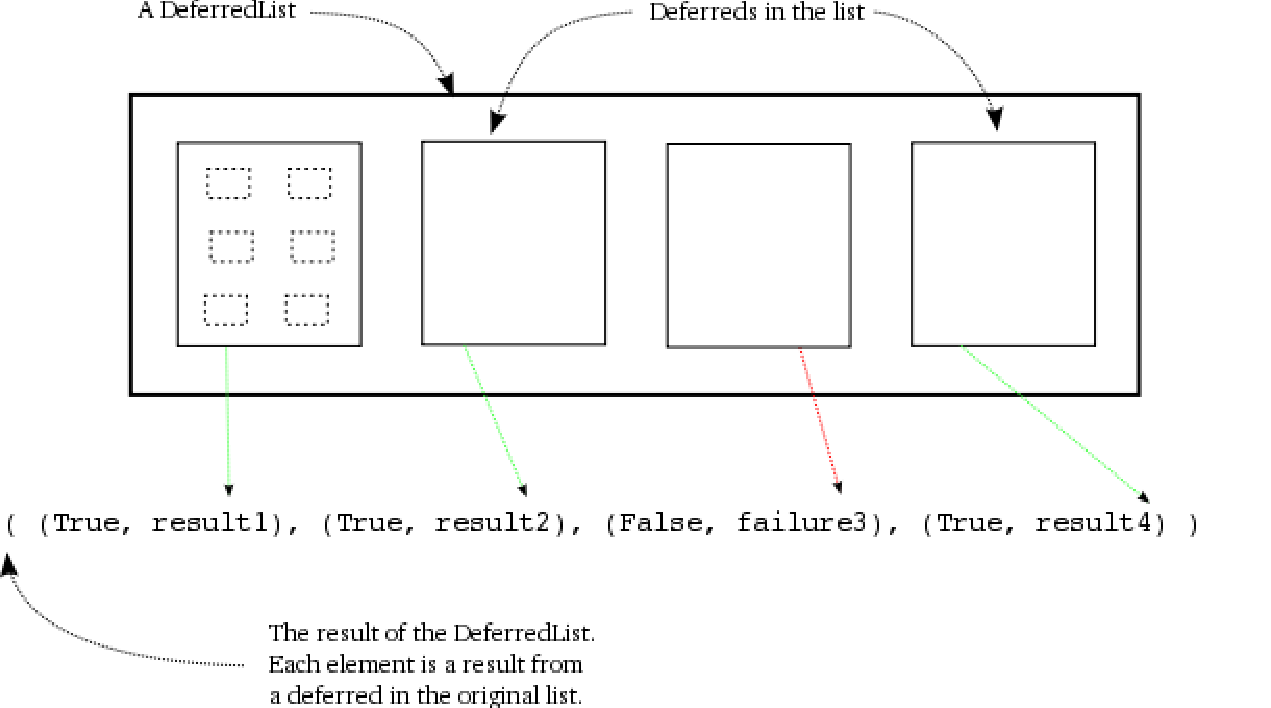
\includegraphics[width=0.8\textwidth]{images/deferred-list.pdf}
    \caption{Результат DeferredList'а\label{fig:deferred-list}}
\end{center}
\end{figure}


Все достаточно просто. Существует несколько опций в DeferredList, 
которые мы не обсудили, и которые меняют поведение того, что 
мы обсудили выше. Мы вернемся к ним позже.


В следующей части мы узучим еще одну особенность класса 
Deferred, которая была недавно добавлена в Twisted 10.1.0.


\subsection{Упражнения}

\begin{enumerate}
\item Прочитайте исходники DeferredList.

\item Поменяйте примеры в deferred-list для экспериментирования с 
    опциями конструктора fireOnOneCallback и fireOnOneErrback. Продумайте 
    ситуации, когда вы бы использовали один или другой аргумент (или оба).

\item Можете ли вы создать DeferredList, используя список DeferredList'ов? 
    Если да, как бы выглядел результат?

\item Поменяйте клиент 8.0 так, чтобы он не ничего не печатал до тех 
    пор, пока все поэмы не скачались. На этот раз вы будете использовать 
    результат из DeferredList.

\item Определите семантику DeferredDict и реализуйте этот класс.

\end{enumerate}

